\section{Logical Clock}\label{sc:logicalClock}

In an absence of real clocks, a logical clock would be applicable to coordinate task and allow ordering of events between nodes in a distributed system. Logical clocks range from mere counters, that periodically increments some integer value, to complex vector time stamps with multiple sets of integer vectors. In this section we look at the need for logical clocks, define a happened-before relation and Lamport scalar time stamps. Time is defined in terms different from \textit{t(x)}

\subsection{A framework for logical clocks}

We define the logical clock as \textit{C} consisting of a time domain \textit{T}. Relation \textit{->} is called the happened-before relation or earlier-than. The logical clock C maps an event e to a element in the time domain T, which we denote as C(e) and define as:

\[ C: E \longmapsto T \]
which satisfies the three properties for the happened-before relation:

\begin{itemize}
	\item Clock consistency: For two events $e_i$ and $e_j$, $e_i$ -> $e_j$ $\Longrightarrow$ C($e_i$) < C($e_j$)
	\item Contrapositive: If C($e_i$) $\nless$ C($e_j$), then $e_i$ $\nrightarrow$ $e_j$
	\item Strong consistency: $e_i$ -> $e_j$ $\Leftrightarrow$ C($e_i$) < C($e_j$)
\end{itemize}

To implement a logical clock in a system of multiple processes, we need to address two issues: A local data structure in each process $p_i$ to represent logical time and a protocol to update the data structures of other processes to ensure the clock consistency condition. This protocol ensures that process $p_j$ local clock and its view on the global clock is consistent, and can be implemented with Lamport time stamps. 

\subsection{Lamport time-stamps}

Invented by Leslie Lamport in 1978, it is an algorithm to order events in a system by using scalar time, a simple non-negative integer $C_i$ time stamp that each process in a system manages. To implement it, we look at at send-scenario, where $p_i$ relays a message to $p_j$.

\begin{itemize}
	\item Before a send event, process $p_i$ executes the following: $C_i$ $\colon$=  $C_i$ + d, where d is a non-zero scalar.
	\item Process $p_i$ sends the message to process $p_j$ containing a payload and the time stamp $C_i$.
	\item Process $p_j$ receives the message with time stamp $C_i$ and executes: $C_j$ $\colon$= max($C_j$,$C_i$) 
\end{itemize}

This ensures that process $p_j$ will update its local logical clock newest global logical clock whenever it receives messages from other processes, allowing events to happen at a more consistent basis now that a given process uses the most up-to-date global clock to know when to fire.

On Figure \ref{fig:lamport}, an example of three processes are given with the lamport timestamp implementation.


\begin{figure}[H]
	\centering
	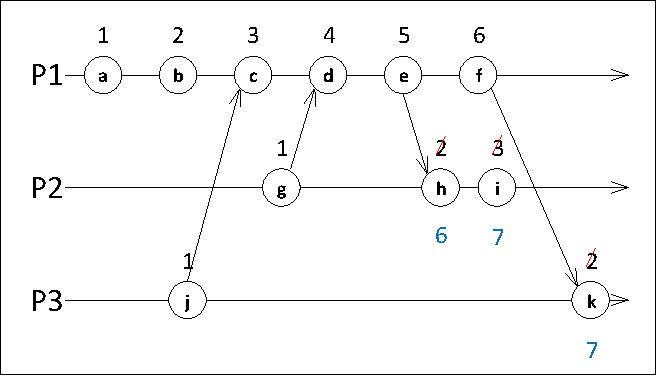
\includegraphics[width=0.3\linewidth]{synchronization/logicalClock/fig/lamport.pdf}
	\caption{An example of the lamport timestamp correction, with three processes \textit{P1}, \textit{P2} and \textit{P3}. Blue numbers are the correction of the lamport timestamps, since $e \rightarrow h$ and $f \rightarrow k$ both were in wrong order.}
	\label{fig:lamport}
\end{figure}
